% Tento soubor nahraďte vlastním souborem s obsahem práce.
%=========================================================================
% Autoři: Michal Bidlo, Bohuslav Křena, Jaroslav Dytrych, Petr Veigend a Adam Herout 2019

% Pro kompilaci po částech (viz projekt.tex), nutno odkomentovat a upravit
%\documentclass[../projekt.tex]{subfiles}
%\begin{document}

\listofdotazy

\chapter{Úvod}\label{kap_uvod}

\chapter{Základy teorie formálních jazyků}\label{kap_teorie}
Základní přehled matematických znalostí potřebných k~pochopení této kapitoly (a~tím i~celé této práce) je popsán například v~\cite{meduna_zemek_2014}, druhá kapitola.

\section{Abeceda, řetězec a jazyk}

\section{Chomského hierarchie}
\section{Bezkontextová gramatika}\label{kap_bkg}
Následující definice převzaty z~\cite{TIN-opora}.
\begin{definition}\label{def_bkg}
    \emph{Bezkontextová gramatika} je čtveřice $G = (N, T, P, S)$, kde:
    \begin{itemize}
        \item $N$ je konečná množina neterminálních symbolů,
        \item $T$ je konečná množina terminálních symbolů,
        \item $P$ je konečná množina přepisovacích pravidel ve tvaru $A \rightarrow x$, $A \in N$ a $x \in (N \cup T)^*$,
        \begin{itemize}[label=$\circ$]
            \item formálně vyjádřeno, množina $P$ přepisovacích pravidel pro bezkontextové gramatiky je podmnožinou kartézského součinu $P \subseteq  N \times (N \cup T)^*$. 
        \end{itemize}
        \item $S \in N$ je výchozí symbol gramatiky.
    \end{itemize}
\end{definition}

\begin{convention}
    Pro označení bezkontextových gramatik bude v~textu dále využívána zkratka BKG.
    Neterminální symboly budou označovány jako neterminály, terminální symboly jako terminály.
\end{convention}

\subsection*{Derivační krok}\label{kap_der_krok}
Myšlenkou derivačního kroku je přepsat aktuální řetězec na řetězec nový za použití pravidla BKG.
\begin{definition}\label{def_derivacni_krok}
    Nechť $G = (N, T, P, S)$ je BKG, $\alpha, \beta  \in (N \cup T)^*$ a $p = A \rightarrow x \in P$. \\
    Mezi řetězci $\alpha$ a~$\beta$ platí binární relace $\underset{G}{\Rightarrow}$, nazývaná \emph{přímá derivace}, jestliže můžeme řetězce $\alpha$ a~$\beta$ vyjádřit ve tvaru
    \begin{align*}
        \alpha &= uAv\\
        \beta &= uxv
    \end{align*}
    kde $u$ a~$v$ jsou libovolné řetězce z~$(N \cup T)^*$. 
    Říká se také, že gramatika $G$ provádí \emph{derivační krok} z~$uAv$ do $uxv$, respektive z~$\alpha$ do $\beta$.
\end{definition}
To znamená, že pokud lze přepsat řetězec $\alpha = uAv$ na řetězec $\beta = uxv$ za použití pravidla $A \rightarrow x$, potom mezi řetězci $\alpha$ a~$\beta$ je relace přímé derivace, zapsáno $\alpha \Rightarrow \beta$.

\begin{figure}[t]
    \centering
    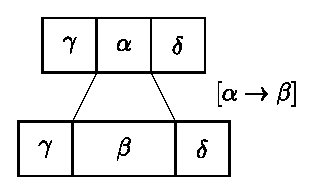
\includegraphics{obrazky-figures/derivacni_krok_bkg.eps}
    \caption{Ilustrace derivačního kroku za použití pravidla $A \rightarrow x$.}
\end{figure}

\subsection*{Sekvence derivačních kroků}\label{kap_sekvence_der_kroku}
\begin{definition}\label{ref_tranz_uzaver}
    Nechť $G = (N, T, P, S)$ je BKG a~$\alpha, \beta \in (N \cup T)^*$. \\
    Mezi řetězci $\alpha$ a $\beta$ platí relace $\Rightarrow^+$ nazývaná \emph{derivace}, jestliže existuje posloupnost přímých derivací $v_{i-1} \Rightarrow v_i, i \in \{1, \ldots, n\}, n \geq 1$ taková, že platí
    \begin{center}
        $\alpha = v_0 \Rightarrow v_1 \Rightarrow \ldots \Rightarrow v_{n-1} \Rightarrow v_n = \beta$.
    \end{center}
    Tato posloupnost se nazývá \emph{derivace délky n}.
    Platí-li $\alpha \Rightarrow \beta$, pak řetězec $\beta$ lze \emph{generovat} z~řetězce $\alpha$, nebo také $\beta$ je \emph{derivovatelný} z~$\alpha$ v~gramatice $G$.
    Relace $\Rightarrow^+$ je tranzitivním uzávěrem relace přímé derivace $\Rightarrow$.
    Symbolem $\Rightarrow^n$ se značí n-tá mocnina přímé derivace $\Rightarrow$.
\end{definition}
Jinými slovy, pokud řetězec $\alpha$ derivuje řetězec $\beta$ v~nenulovém počtu kroků a~zároveň $\beta$ derivuje řetězec $\gamma$ v~nenulovém počtu kroků, pak je zřejmé, že $\alpha$ derivuje $\gamma$ v~nenulovém počtu kroků, zapsáno $\alpha \Rightarrow^+ \gamma$. 

\begin{definition}\label{def_refl_uzaver}
    Nechť $G = (N, T, P, S)$ je BKG a~$\alpha, \beta \in (N \cup T)^*$. \\
    Jestliže v~$G$ platí pro řetězce $\alpha$ a~$\beta$ relace $\alpha \Rightarrow^+ \beta$ nebo identita $\alpha = \beta$, pak $\alpha \Rightarrow^* \beta$.
    Relace~$\Rightarrow^*$ je reflexivním a~tranzitivním uzávěrem relace přímé derivace $\Rightarrow$.  
\end{definition}
Reflexivní uzávěr relace přímé derivace $\Rightarrow$ znamená, že řetězec přímo derivuje sám sebe v~nula krocích.
Také je možné říci, že se nepoužije žádné pravidlo k~přepsání řetězce na sebe sama, zapsáno $\alpha \Rightarrow^0 \alpha$.


\section{Konečný automat}
Definice související s~konečnými automaty převzaty z~\cite{meduna2023automata}, není-li řečeno jinak.
\begin{definition}\label{def_konecny_automat}
    \emph{Konečný automat} je pětice
    \begin{equation*}
        M = (Q, \Sigma, R, s, F),
    \end{equation*}
    kde
    \begin{itemize}
        \item $Q$ je konečná množina stavů,
        \item $\Sigma$ je konečná vstupní abeceda, $Q \cap \Sigma = \emptyset$,
        \item $R$ je konečná relace, $R \subseteq Q \times (\Sigma \cup \{\varepsilon\}) \times Q$,
        \begin{itemize}[label=$\circ$]
            \item je nazývána \emph{množinou pravidel} ve tvaru $qa \rightarrow p,\; q, p \in Q,\;a \in \Sigma \cup \{\varepsilon\}$.
            Jakákoli uspořádaná trojice $(q, a, p) \in R$ je pravidlem, zapsáno $qa \rightarrow p$.
            \item Další možnost zápisu je zobrazení (\emph{přechodová funkce}) $R: Q \times \Sigma \rightarrow 2^Q$ \cite{TIN-opora}.
        \end{itemize}
        \item $s \in Q$ je počáteční stav automatu,
        \item $F \subseteq Q$ je konečná množina koncových stavů. 
    \end{itemize}
\end{definition}

\begin{convention}
    Pro označení konečných automatů bude dále v~textu použito zkrácené KA. 
\end{convention}

U~konečných automatů popisujeme jejich \emph{konfiguraci}\,--\,ve kterém stavu se nachází a~jaký řetězec na vstupní pásce.
\begin{definition}\label{def_konfigurace_ka}
    Nechť $M = (Q, \Sigma, R, s, F)$ je KA. Dle autorů v~\cite{TIN-opora} je konfigurace $M$ uspořádaná dvojice
    \begin{equation*}
        (q, w) \in Q \times \Sigma^*.
    \end{equation*} 
    Nechť $X_M$ značí množinu všech konfigurací $M$.
\end{definition}

Pomocí konfigurací můžeme definovat \emph{přechody} KA, které reprezentují jejich výpočetní kroky.
Výpočetní krok znamená přechod z~jedné konfigurace do druhé za přečtení symbolu ze vstupní pásky.
\begin{definition}\label{def_prechod_ka}
    Nechť $M = (Q, \Sigma, R, s, F)$ je KA.\\
    Binární relace $\vdash_{\scriptscriptstyle M}$, nazývána přechodem KA $M$, je
    \begin{equation*}
        \beta\; \vdash_{\scriptscriptstyle M}\chi,
    \end{equation*}
    kde $\beta = (q, ax),\, \chi = (p, x) \in X_M,$ a~$qa \rightarrow p \in R$.
    Je to binární relace na množině konfigurací\,--\,pokud $\beta\, \vdash_{\scriptscriptstyle M} \chi$, pak $(\beta, \chi) \in X_M \times X_M$.
    Pokud $a = \varepsilon$, není ze vstupní pásky přečten žádný symbol.
    
    Symboly $\vdash_{\scriptscriptstyle M}^n, \vdash_{\scriptscriptstyle M}^+$ a~$\vdash_{\scriptscriptstyle M}^*$ nechť značí příslušně $n$-tou mocninu pro $n \geq 0$, tranzitivní a reflexivně-tranzitivní uzávěr relace $\vdash_{\scriptscriptstyle M}$ podobně jako u~derivačního kroku BKG (\ref{def_derivacni_krok}), čímž reprezentují \emph{sekvenci přechodů} KA $M$.
    Například pro konfigurace $\beta$ a~$\chi$ platí $\beta\; \vdash_{\scriptscriptstyle M}^+ \chi$ právě tehdy, když
    \begin{equation*}
        \beta = c_0 \vdash_{\scriptscriptstyle M} c_1 \vdash_{\scriptscriptstyle M} \ldots \vdash_{\scriptscriptstyle M} c_{n-1} \vdash_{\scriptscriptstyle M} c_{n} = \chi,
    \end{equation*}
    pokud $\beta, \chi, c_1, \ldots, c_{n-1} \in X_M,\; n \geq 1$.
\end{definition}

\begin{convention}
    Bude-li z~kontextu jasné, že se jedná o~přechod automatu~$M$, pak bude relace přechodu $\vdash$ psána bez indexu $M$.  
\end{convention}

\begin{definition}
    Nechť $M = (Q, \Sigma, R, s, F)$ je KA.\\
    Jazyk přijímaný $M$, značen $L(M)$, je
    \begin{equation*}
        L(M) = \{w \in \Sigma^*: sw\; \vdash^* f,\; f \in F\}.
    \end{equation*}
    Jsou to řetězce takové, po jejichž zpracování skončí $M$ v~koncovém stavu.
\end{definition}


\begin{definition}
    Nechť $M = (Q, \Sigma, R, s, F)$ je KA.\\
    $M$ je \emph{KA bez $\varepsilon$-přechodů}, pokud pro každé pravidlo $qa \rightarrow p \in R$ platí, že $a \neq \varepsilon$.
\end{definition}

\begin{definition}
    Nechť $M = (Q, \Sigma, R, s, F)$ je KA bez $\varepsilon$-přechodů.\\
    $M$ je \emph{deterministický KA} právě tehdy, když pro každé $q \in Q$ a~každé $a \in \Sigma$ neexistuje více než jedno $p \in Q$ takové, že $qa \rightarrow p \in R$.
    Jinými slovy, z~jednoho stavu není možné přejít do několika stavů přečtením stejného symbolu.
\end{definition}

\section{Zásobníkový automat}\label{kap_zasobnikovy_automat}
Zásobníkový automat je rozšíření konečného automatu, popsaného v~definici \ref{def_konecny_automat}, o~zásobník.
Zásobník slouží jako paměťové médium, na které si automat může ukládat informace v~podobě symbolů zásobníkové abecedy.
Následující definice převzaty z~\cite{meduna2023automata, TIN-opora}.
\begin{definition}\label{def_zasobnikovy_automat}
    \emph{Zásobníkový automat} (ZA) je sedmice 
    \begin{center}
        $M = (Q, \Sigma, \Gamma, R, s, S, F)$,
    \end{center}
    kde:
    \begin{itemize}
        \item $Q, \Sigma, s, F$ jsou definovány stejně jako v~definici \ref{def_konecny_automat},
        \item $\Gamma$ je konečná zásobníková abeceda,
        \item $R$ je konečná relace $R \subseteq \Gamma \times Q \times (\Sigma \cup \{\varepsilon\}) \times \Gamma^* \times Q$ nazývána množinou pravidel ZA,
        \begin{itemize}[label=$\circ$]
            \item každé pravidlo $(A, q, a, w, p)$ může být zapsáno ve tvaru $Aqa \rightarrow wp$, kde $A \in \Gamma,$ $q, p \in Q,\; a \in \Sigma \cup \{\varepsilon\},\; w \in \Gamma^*$ \cite{meduna2017modely},
        \end{itemize}  
        \item $S \in \Gamma$ je počáteční symbol na zásobníku.
    \end{itemize}
\end{definition}

\begin{convention}
    Zásobníkové automaty budou dále značeny zkráceně ZA.
\end{convention}

\begin{definition}\label{def_konfigurace_za}
    Nechť $M = (Q, \Sigma, \Gamma, R, s, S, F)$ je ZA.\\
    Konfigurací ZA nazveme trojici
    \begin{equation*}
        (\alpha, q, w) \in \Gamma^* \times Q \times \Sigma^*, 
    \end{equation*}
    kde
    \begin{itemize}
        \item $\alpha$ je obsah zásobníku,
        \item $q$ je aktuální stav automatu (\emph{řídící jednotky}),
        \item $w$ je doposud nepřečtená část vstupního řetězce, jehož první symbol je aktuálně pod čtecí hlavou.
        Pokud $w = \varepsilon$, všechny symboly byly ze vstupní pásky již přečteny.
    \end{itemize}
    Nechť $X_M$ reprezentuje množinu všech konfigurací ZA $M$.
\end{definition}

\begin{definition}\label{def_prechod_za}
    Nechť $M = (Q, \Sigma, \Gamma, R, s, S, F)$ je ZA.\\
    Přechod ZA je binární relace definována nad množinou konfigurací (podobně jako v~definici \ref{def_prechod_ka}) v~podobě
    \begin{equation*}
        \beta\; \vdash \chi,
    \end{equation*}
    kde $\beta = (uA, q, av),\; \chi = (uw, p, v)$ a~$Aqa \rightarrow wp \in R$.
    Symbolem $A$ je reprezentován vrchol zásobníku a~symbol $a$ nechť reprezentuje aktuální symbol pod čtecí hlavou.
    Pokud $w = \varepsilon$, pak se pouze vyjme $A$ ze zásobníku bez náhrady.
    Relace $\vdash^n,\; \vdash^+,\; \vdash^*$ jsou opět $n$-tou mocninou relace, tranzitivním a~reflexivně-tran\-zi\-tiv\-ním uzávěrem.
\end{definition}
Oproti klasickým KA se při přechodu musí pracovat se zásobníkem, ze kterého se vyjme symbol $A$, namísto něj se vloží symbol $w$.

Automat $M$ přijímá řetězec právě tehdy, když $Ssw \vdash^* uf$ v~$M;$ $u \in \Gamma^*, f \in F$.
\begin{definition}\label{def_jazyk_za}
    Nechť $M = (Q, \Sigma, \Gamma, R, s, S, F)$ je ZA.\\
    Jazyk přijímaný $M$ je
    \begin{equation*}
        L(M) = \{w : w \in \Sigma^*,\; Ssw \vdash^* f,\; f \in F\}.
    \end{equation*}
\end{definition}

\begin{example}\label{example_za}
    Nechť $M = (\{s, f\}, \{a, b\}, \{S, a\}, R, s, S, \{f\})$ je ZA a 
    \begin{equation*}
        R = \{Ssa \rightarrow as,\; asas \rightarrow aas,\; asb \rightarrow f,\; afb \rightarrow f\}.
    \end{equation*}
    Počáteční konfigurace nechť je $(S, s, aaabbb)$.
    Přechody $M$ budou vypadat následovně:
    \begin{alignat*}{2}
        (S, s, aaabbb) &\vdash (a, s, aabbb) \quad && [Ssa \rightarrow as] \\
                       &\vdash (aa, s, abbb) \quad && [asa \rightarrow aas] \\
                       &\vdash (aaa, s, bbb) \quad && [asa \rightarrow aas] \\
                       &\vdash (aa, f, bb) \quad   && [asb \rightarrow f] \\ 
                       &\vdash (a, f, b) \quad      && [afb \rightarrow f] \\
                       &\vdash (\varepsilon, f, \varepsilon) \quad && [afb \rightarrow f]
    \end{alignat*}
\end{example}

\subsection*{Rozšířený zásobníkový automat}\label{kap_rozsireny_ZA}
Rozšířené zásobníkové automaty reprezentují přirozené rozšíření klasických ZA, které na zásobníku mohou pracovat pouze s~jeho vrcholem.
Rozšířené zásobníkové automaty mohou provádět expanzi symbolů na zásobníku v~libovolné hloubce, jinak pracují indenticky.
Text a~definice v~této kapitole převzaty z~\cite{meduna2023automata, meduna_zemek_2014}, není-li řečeno jinak.

\begin{definition}\label{def_rza}
    \emph{Rozšířený zásobníkový automat} (RZA) je sedmice
    \begin{center}
        $M = (Q, \Sigma, \Gamma, R, s, S, F)$,
    \end{center}
    kde:
    \begin{itemize}
        \item $Q, \Sigma, s, S, F$ jsou definovány stejně jako u~klasických ZA (\ref{def_zasobnikovy_automat}),
        \item $\Gamma$ je zásobníková abeceda, $\mathbb{N},\; Q,$ a~$\Gamma$ jsou navzájem disjunktní, $\Sigma \subseteq \Gamma$\dotaz{opravdu $\subseteq$ a ne $\subset$?}  a~$\Gamma \setminus \Sigma$ obsahuje speciální symbol $\#$ (\emph{spodní symbol}), který je považován za dno zásobníku, 
        \item $R$ je konečná relace
        \begin{alignat*}{-1}
             &(\mathbb{N} \times Q \,\times \,&& (\Gamma \setminus (\Sigma \cup \{\#\})) &&\times Q \times (\Gamma \setminus \{\#\})^+) \;\cup \\
             &(\mathbb{N} \times Q \,\times \,&& \{\#\} &&\times Q \times (\Gamma \setminus \{\#\})^*\{\#\}),
        \end{alignat*}
        místo uspořádané pětice $(m, q, A, p, v) \in R$ píšeme $mqA \rightarrow pv \in R$ a~$R$ nazýváme množinou pravidel.
        \begin{itemize}[label=$\circ$]
            \item Z definice $R$ lze vidět, že jsou dva typy přechodových pravidel, dají se zapsat ve tvaru
            \begin{align*}
                mqA  &\rightarrow pv,\\
                mq\# &\rightarrow pv\# \; \cite{meduna_rgd_pda}.
            \end{align*}
            O~jejich použití a~rozdílech je psáno v~definici \ref{def_prechod_rza}.
        \end{itemize}
    \end{itemize}
\end{definition}

\begin{convention}
    Rozšířené zásobníkové automaty budou dále označeny zkratkou RZA.
\end{convention}

Přechody RZA pracují, stejně jako přechody ZA, nad konfiguracemi.
Konfigurace jsou podobné těm u~klasických ZA, nicméně stav zásobníku musí končit symbolem $\#$ a~zbytek řetězce na zásobníku jej nesmí obsahovat. 
\begin{definition}\label{def_konfigurace_za}
    Nechť $M = (Q, \Sigma, \Gamma, R, s, S, F)$ je RZA.\\
    Konfigurací RZA nazveme trojici
    \begin{equation*}
        (q, w, \alpha) \in Q \times \Sigma^* \times (\Gamma \setminus \{\#\})^*\{\#\}.
    \end{equation*}
    Nechť $X_M$ reprezentuje množinu všech konfigurací RZA $M$.
\end{definition}

Další podobnost je práce s~řetězci abedecedy $\Sigma$ a~s~pravidly při přechodech. 
Jediná změna od klasických ZA již byla zmíněna na začátku této kapitoly\,--\,při přechodech se na vrcholu zásobníku mohou měnit celé řetězce.

\begin{definition}\label{def_prechod_rza}
    Nechť $M = (Q, \Sigma, \Gamma, R, s, S, F)$ je RZA a~$\beta,\; \chi \in X_M$ jeho konfigurace.\\
    $M$ vyjme (anglicky \emph{pops}) ze zásobníku symbol a~přejde z~konfigurace $\beta$ do konfigurace $\chi$ za přečtení symbolu vstupní pásky, symbolicky zapsáno
    \begin{equation*}
        \beta\, \prescript{}{p}{\vdash}\; \chi,
    \end{equation*}
    pokud konfigurace jsou ve tvaru $\beta = (q, au, az),\; \chi = (q, u, z),\; a \in \Sigma$, $u \in \Sigma^*$, ${z \in \Gamma^*}$.
    $M$ rozšíří (anglicky \emph{expands}) symbol na zásobníku a~přejde z~konfigurace $\beta$ do konfigurace $\chi$ za přečtení symbolu ze vstupní pásky, symbolicky zapsáno
    \begin{equation*}
        \beta\, \prescript{}{e}{\vdash}\; \chi,
    \end{equation*} 
    pokud konfigurace jsou ve tvaru $\beta = (q, w, uAz),\; \chi = (p, w, uvz)$ a~zároveň $mqA \rightarrow pv \in R$; $q, p \in Q$, $w \in \Sigma^*$, $A \in \Gamma$, $u, v, z \in \Gamma^*$; $m$ je hloubka symbolu $A$ v~zásobníku, respektive $u$ obsahuje $m-1$ \emph{nevstupních} symbolů (symboly $a$, pro které platí $\{a\, :\, a \in \Gamma \setminus \Sigma\}$). 
    Pro ilustraci, že automat udělá přechod $\beta\, \prescript{}{e}{\vdash}\; \chi$ podle pravidla $mqA \rightarrow pv$, píšeme
     \begin{equation*}
        \beta\, \prescript{}{e}{\vdash}\; \chi \ \; [mqA \rightarrow pv].
    \end{equation*}
    $M$ udělá \emph{přechod} z~$\beta$ do $\chi$, psáno
    \begin{equation*}
        \beta\, \vdash\, \chi
    \end{equation*}
    právě tehdy, když $M$ udělá vyjmutí symbolu $\beta\, \prescript{}{p}{\vdash}\; \chi$ nebo expanzi symbolu $\beta\, \prescript{}{e}{\vdash}\; \chi$.
    Tranzitivní uzávěry $\prescript{}{p}{\vdash^+}, \prescript{}{e}{\vdash^+}$, reflexivně-tranzitivní uzávěry $\prescript{}{p}{\vdash^*}, \prescript{}{e}{\vdash^*}$ a~$n$-té mocniny $\prescript{}{p}{\vdash^n}, \prescript{}{e}{\vdash^n}$ jsou definovány standardně.
    Alternativní definice přechodu je popsána v~\cite{TIN-opora}.
\end{definition}
\begin{figure}[ht]
    \caption{\todo{obrazek p-prechodu a e-prechodu rza}}\label{fig_prechod_rza}
\end{figure}

Pokud existuje $n \in \mathbb{N}$ takové, že pro všechna pravidla $M$ platí, že jejich hloubka je maximálně rovna $n$, pak říkáme, že $M$ je hloubky maximálně $n$, zapsáno $\prescript{}{n}{M}$.

\begin{definition}\label{def_jazyk_rza}
    Nechť $\prescript{}{n}{M} = (Q, \Sigma, \Gamma, R, s, S, F)$ je RZA hloubky $n \in \mathbb{N}$. \\
    Jazyk přijímaný automatem $M$ je
    \begin{equation*}
        L(\prescript{}{n}{M}) = \{w \in \Sigma^*: (s, w, S\#) \vdash^* (f, \varepsilon, \#) \text{ v } \prescript{}{n}{M},\; f \in F\}.
    \end{equation*}
\end{definition}

Tyto jazyky jsou přijímané vyprázdněním zásobníku a~zároveň přechodem do koncového stavu automatu.
Dále existují jazyky přijímané RZA pouze vyprázdněním zásobníku, přičemž automat se nemusí dostat do koncového stavu.

\begin{definition}\label{def_jazyk_rza_empty}
    Nechť $\prescript{}{n}{M} = (Q, \Sigma, \Gamma, R, s, S, F)$ je RZA hloubky $n \in \mathbb{N}$. \\
    Jazyk přijímaný automatem M vyprázdněním zásobníku je
    \begin{equation*}
        E(\prescript{}{n}{M}) = \{w \in \Sigma^* : (s, w, S\#) \vdash^* (q, \varepsilon, \#) \text{ v~}\prescript{}{n}{M},\; q \in Q\}.
    \end{equation*}
\end{definition}

\begin{example}\label{example_rza}
    Nechť $\prescript{}{2}{M} = (\{s, q, p, f\}, \{a, b, c\}, \Sigma \cup \{A, S, \#\}, R, s, S, \{f\})$, kde $R$ je
    \begin{alignat*}{3}
        & 1sS \rightarrow qAA, \qquad \qquad && 1qA \rightarrow fab, \qquad \qquad && 1fA \rightarrow fc, \\
        & 1qA \rightarrow paAb, \qquad \qquad && 2pA \rightarrow qAc. \qquad \qquad &&
    \end{alignat*}
    Mějme počáteční konfiguraci $(s, aabbcc, S\#)$.
    $M$ udělá nejdříve dvakrát expanzi\,--\,jednou expanduje startovací symbol na $AA$, přičemž $A$ není vstupní symbol, takže expanze proběhne podruhé.
    \begin{alignat*}{2}
        (s, aabbcc, S\#)\, &\prescript{}{e}{\vdash}\; (q, aabbcc, AA\#) \quad && [1sS \rightarrow qAA] \\
                           &\prescript{}{e}{\vdash}\; (p, aabbcc, aAbA\#) \quad && [1qA \rightarrow paAb] \\
    \end{alignat*}
    Na aktuální konfiguraci je vidět, že na vrcholu zásobníku i~aktuálně čtený symbol je $a$.
    $M$ tento symbol vyjme.
    \begin{equation*}
        (p, aabbcc, aAbA\#)\, \prescript{}{p}{\vdash}\; (p, abbcc, AbA\#)
    \end{equation*}
    Následující krok bude znovu expanze, tentokrát hlouběji v~zásobníku.
    \begin{equation*}
        (p, abbcc, AbA\#)\, \prescript{}{e}{\vdash}\; (q, abbcc, AbAc\#) \quad [2pA \rightarrow qAc]
    \end{equation*}
    Dále přijímání řetězce probíhá stejným způsobem jako v předešlých krocích.
    \dotaz{Příklad v knize - přeskočení kroku z 5 na 6, z kroku 7 na 8 je psána expanze, ale nic se v konfiguraci nezměnilo - vysvětlím osobně}
    \begin{alignat*}{2}
        (q, abbcc, AbAc\#)\, &\prescript{}{e}{\vdash}\; (q, abbcc, abbAc\#) \quad && [1qA \rightarrow fab] \\
                             &\prescript{}{p}{\vdash}\; (f, bbcc, bbAc\#) \quad && \\
                             &\prescript{}{p}{\vdash}\; (f, bcc, bAc\#) \quad && \\
                             &\prescript{}{p}{\vdash}\; (f, cc, Ac\#) \quad && \\
                             &\prescript{}{e}{\vdash}\; (f, cc, cc\#) \quad && [1fA \rightarrow fc] \\ 
                             &\prescript{}{p}{\vdash}\; (f, c, c\#) \quad && \\
                             &\prescript{}{p}{\vdash}\; (f, \varepsilon, \#) \quad &&
    \end{alignat*}
\end{example}

\chapter{Důležité pojmy syntaktické analýzy}\label{5_teorie_sa}

\section{Množiny potřebné k~sestrojení LL tabulky}

\section{LL tabulka}

\section{Prediktivní syntaktická analýza}

\section{Precedenční tabulka}

\section{Precedenční syntaktická analýza}

\section{Abstraktní syntaktický strom}


\chapter{Gramatické systémy}\label{kap_GS}

Veškeré definice a znalosti použité v~této kapitole převzaty z~\cite{CDGS, PCGS, Handbook-Of-Formal-Languages-2}, není-li řečeno jinak.
\dotaz{Jak uvést tuto kapitolu?}

\section{Kooperující distribuované gramatické systémy}\label{kap_CDGS}

Kooperující distribuovaný (\emph{cooperating distributed}) gramatický systém stupně~\emph{n}~je systém gramatik, které mezi sebou sdílejí množinu neterminálů i~terminálů a~startovací symbol.
Spolupracují mezi sebou předáváním řízení derivace aktuálně zpracovávaného řetězce dle pravidel nastaveného \emph{derivačního režimu}.

\begin{definition}\label{def_cdgs}
\text{Kooperující distribuovaný gramatický systém je $(n+3)$-tice}
\begin{center}
    $\Gamma = (N, T, S, P_1, \ldots ,P_n)$,
\end{center}
kde:
\begin{itemize}
    \item $N$, $T$, a $S$ jsou definovány stejně jako v~definici \ref{def_bkg},
    \item $P_i$ je konečná množina pravidel ve tvaru $A\rightarrow x$, kde pravidla jsou definována stejně jako v~definici \ref{def_bkg}, nazývaná \emph{komponentou} systému, $i \in \{1, \ldots, n\}$,
    \item $i$-tá gramatika systému se zapisuje jako $G_i = (N,T,S,P_i)$
\end{itemize}   
Alternativní definice pro CDGS je $\Gamma = ((N, T, S, P_1), \ldots , (N, T, S, P_n))$.
\end{definition}

\begin{convention}
    Pro označení kooperujících distribuovaných gramatických systémů bude dále využito zkrácené \emph{CDGS}, případně \emph{CD gramatické systémy}.
\end{convention}

\subsection*{Derivační krok v~CDGS}
Notace derivačního kroku v~CDGS je
\begin{center}
    $x \prescript{}{i}{\Rightarrow}^{f} y$.
\end{center}
Tento zápis znamená, že řetězec $x \in (N \cup T)^{*}$ derivuje řetězec $y \in (N \cup T)^{*}$ v~$i$-té komponentě za použití \emph{derivačního režimu} $f$.

\subsubsection*{Derivační režimy}

Prvním příkladem je režim $*$, který byl v~definici \ref{def_refl_uzaver} uveden pro bezkontextovou gramatiku a~princip v~CD gramatických systémech je podobný.
Při použití tohoto derivačního režimu řetězec $x \in (N \cup T)^*$ derivuje řetězec $y \in (N \cup T)^*$ v~libovolném počtu kroků v~$i$-té komponentě, zapsáno $x \prescript{}{i}{\Rightarrow}^{*}y$.
Je možné předat řízení derivace jiné komponentě i~v~případě, že ve stejné komponentě lze s~derivací stejného řetězce pokračovat.

Podobným příkladem je režim \emph{ukončovací}, který spočívá v~nutné derivaci řetězce v~dané komponentě, dokud je to možné. Značí se písmenem \emph{t}. Jsou dvě nutné podmínky, aby \emph{y} bylo derivovatelné z~\emph{x} v~komponentě $G_i$ režimem \emph{t}.
\begin{enumerate}
    \item $x\; \prescript{}{i}{\Rightarrow}^{*}\; y$\,--\,v~dané komponentě lze posloupností derivačních kroků získat řetězec $y$ z~řetězce $x$,
    \item $y\; \prescript{}{i}{\nRightarrow}\;\,z$ pro všechna $z \in (N \cup T)^{*}$\,--\,ve stejné komponentě nelze nalézt další pravidlo, které by derivovalo $y$.
\end{enumerate}
Jinými slovy, pokud můžeme z~aktuálního řetězce v~aktuální komponentě odvodit řetězec nový, \emph{musí} se s~derivací v~této komponentě pokračovat. 

Další derivační režimy:
\begin{itemize}
    \item alespoň \emph{k}~derivací, tedy $x\; \prescript{}{i}{\Rightarrow}^{\geq k}\ y$,
    \item nejvíce \emph{k}~derivací, tedy $x\; \prescript{}{i}{\Rightarrow}^{\leq k}\ y$,
    \item právě \emph{k}~derivací, tedy $x\; \prescript{}{i}{\Rightarrow}^{=k}\ y$,
\end{itemize}
kde $k \in \mathbb{N} \cup \{0\}$ a $i$ symbolizuje $i$-tou komponentu gramatického systému.

Derivačních režimů existuje mnohem více\dotaz{Zdroj?? - Mluvili jsme o~tom na konzultaci a říkáte to i v~záznamu přednášky TID. Stačil by asi klidně jen nějaký odkaz na výčet. }, nejsou ale pro tuto práci podstatné.
Tyto režimy mohou být reprezentovány jako množina, což pomůže definovat další pojmy v~následující podkapitole o~generovaném jazyce.
\begin{definition}\label{def_der_rezimy}
    Nechť $k\in \mathbb{N}$ a $*$, $t$ představují derivační režimy. \\
    Potom množina
    \begin{center}
        $D = \{*, t\} \cup \{\leq k, \geq k, =k\}$ 
    \end{center}        
    reprezentuje derivační režimy použitelné v~CD gramatických systémech.
\end{definition}

\subsection*{Jazyk generovaný CD gramatickým systémem}
Než bude definován samotný jazyk, je vhodné definovat pomocnou množinu, která reprezentuje \emph{možné derivace} z~řetězců.
\begin{definition}\label{def_mozne_derivace}
    Nechť $\Gamma = (N, T, S, P_1, \ldots, P_n)$. \\  
    Potom 
    \begin{center}
        $F(G_j,u,f)=\{v:u_j\Rightarrow^{f}v\},$ $j \in \{1, \ldots, n\},$ $f\in D,$ $u\in (N \cup T)^{*}$
    \end{center}        
    je množina všech řetězců $v$ derivovatelných z~$u$ v~$j$-té komponentě za použití derivačního režimu $f$.
\end{definition}

\begin{definition}\label{def_generovany_jazyk}
    Nechť $\Gamma = (N, T, S, P_1, \ldots, P_n)$. \\  
    Jazyk generovaný systémem $\Gamma$ za derivačního režimu $f$ je 
    \begin{align*}
         L_f(\Gamma) = \{&w \in T^*: \text{ existují } v_0, v_1,\ldots, v_m \text{ takové, že } v_k \in F(G_{j_{k}},v_{k-1}, f),\\
         &k \in \{1, \ldots, m\},\;j_k \in \{1, \ldots, n\},\;v_0 = S,\;v_m = w \text{ pro } m \geq 1\}.
    \end{align*}        
\end{definition} 

Výsledný řetězec $w$, který vznikl postupnou derivací startovacího symbolu $v_0$.
Měl několik mezikroků, které jsou reprezentovány řetězci $v_1, \ldots, v_{m-1}$.
Každý řetězec $v_k$, kde $k \in \{1, \ldots, m\}$ byl zderivován z~řetězce $v_{k-1}$ v~komponentě $G_{j_{k}}$, kde $j_k \in \{1, \ldots, n\}$, za derivačního režimu $f$.

\begin{example}
    Nechť $\Gamma = (\{S, A\}, \{a\}, S, P_1, P_2, P_3)$, kde $P_1 = \{S \rightarrow AA\}$, $P_2 = \{A \rightarrow S\}$, $P_3 = \{A \rightarrow a\}$.
    Nechť $f = t$, $\Gamma$ pracuje na ukončovacím derivačním režimu.

    Počáteční řetězec je počáteční symbol, tedy $S$. 
    Je pouze jedna možnost, jak $S$~přepsat, a~to použitím pravidla z~$P_1$, $S \rightarrow AA$.
    \begin{equation*}
        S \rightarrow AA \quad [S \rightarrow AA]
    \end{equation*}
    Díky tomu, že v~komponentě $P_1$ už neexistuje pravidlo, kterým by mohla derivace dále pokračovat, řízení derivace je předáno komponentě jiné.
    Aktuálně zpracovávaný řetězec je $AA$.
    Komponenty $P_1$ a~$P_2$ mají pravidla pro přepsání neterminálu $A$.
    Při použití derivačního režimu \emph{t} je zřejmé, že celý řetězec bude přepisovat pouze jedna komponenta.
    Při předání komponentě $P_3$ je řetězec přepsán na $aa$,
    \begin{alignat*}{-1}
        AA \rightarrow&&\; aA \quad &&[A \rightarrow a] \\
        aA \rightarrow&&\; aa \,\quad &&[A \rightarrow a]
    \end{alignat*}
    komponenta $P_2$ stejný řetězec přepíše na $SS$.
    \begin{alignat*}{-1}
        AA  \rightarrow&&\; SA && \quad [A~\rightarrow S] \\
        SA  \rightarrow&&\; SS && \quad [A~\rightarrow S] 
    \end{alignat*}
    \begin{alignat*}{-1}
         SS \rightarrow&&\; AAS  \hphantom{A} \quad  &&[S \rightarrow AA] \\ 
        AAS \rightarrow&&\; AAAA \quad &&[S \rightarrow AA]
    \end{alignat*}
    Ze startovacího symbolu dostaneme buď terminál $a$ nebo dva startovací symboly.
    To znamená, že pokaždé, kdy se $AA$ přepíše na $SS$, počet terminálů $a$ se zdvojnásobí.
    Jazyk generovaný systémem $\Gamma$ za derivačního režimu \emph{t}, $L(\Gamma)_t = \{a^{2^n},$ $n \geq 1 \}$.
\end{example}

\subsection*{Klasifikace skupin CD jazyků}
CD jazyky jsou jazyky, které jsou generovány CD gramatickými systémy.
Tyto jazykové rodiny se rozdělují podle různých typů použitých CDGS.
Jejich označení je
\begin{center}
    $CD^y_x(f)$,
\end{center}
kde:
\begin{itemize}
    \item $y$ určuje použití $\varepsilon$-pravidel: 
    \begin{itemize}[label=$\circ$]
        \item $y = \varepsilon$\,--\,$\varepsilon$-pravidla v~komponentách jsou povolena,
        \item $y$ chybí\,--\,$\varepsilon$-pravidla se v~komponentách nemohou vyskytovat,
    \end{itemize}
    \item $x$ je stupeň gramatického systému:
    \begin{itemize}[label=$\circ$]
        \item $n, n \geq 1$\,--\,gramatický systém může obsashovat maximálně $n$~komponent,
        \item $\infty$\,--\,gramatický systém nemá omezen počet komponent,
    \end{itemize}
    \item $f$ je derivační režim, $f \in D$.
\end{itemize}
\begin{example}
    $CD^\varepsilon_6 (t)$ je rodina jazyků generována CD gramatickými systémy s~maximálně šesti komponentami, povolenými $\varepsilon$-pravidly a~pracujícími nad ukončovacím režimem. 
\end{example}

\subsection*{Hybridní CD gramatické systémy}
Hybridní CD gramatické systémy nabízí možnost definovat derivační režim samostatně pro jednotlivé komponenty systému.
\begin{definition}
    \emph{Hybridní CDGS} je n-tice $\Gamma = (N, T, S, (P_1, f_1), \ldots, (P_n, f_n))$, kde:
    \begin{itemize}
        \item $N, T, P_i, S$ jsou definovány stejně jako v~klasických CDGS (\ref{def_cdgs}),
        \item $f_i$ je derivační režim $i$-té komponenty, $f_i \in D$ pro všechna $i \in \{1, \ldots, n\}$.
    \end{itemize}
\end{definition}

Jazyk generovaný těmito gramatickými systémy je velmi podobný jazykům generovaným klasickými CDGS.
Jediný rozdíl je v~použití derivačního režimu příslušné komponenty, který je v~definici označen jako $f_{j_k}$, místo společného derivačního režimu pro celý gramatický systém.
\begin{definition}
    Nechť $\Gamma = (N, T, S, (P_1, f_1), \ldots, (P_n, f_n))$.\\
    Jazyk generovaný systémem $\Gamma$,
    \begin{align*}
        L(\Gamma) = \{&w \in T^*: \text{existují } v_0, v_1,\ldots, v_n \text{ takové, že } v_k \in F(G_{j_k}, v_{k-1}, f_{j_k}),\\
        &k \in \{1, \ldots, m\}, j_k \in \{1, \ldots, n\}, v_0 = S, v_m = w \text{ pro } m \geq 1\}.
    \end{align*}
\end{definition}

Zápis jazykových skupin generovaných hybridními CDGS je
\begin{center}
    $X\,CD^y_{x, v}(f) $, 
\end{center}
kde:
\begin{itemize}
    \item $x, y, f$ jsou definovány stejně jako u~nehybridních CDGS,
    \item $v$ je nepovinné omezení počtu pravidel v~komponentách:
    \begin{itemize}[label=$\circ$]
        \item \emph{m}\,--\,každá komponenta $P_i, i \in \{1, \ldots, n\}$ obsahuje nejvíce $m$ pravidel, $m \geq 1$,
        \item $\infty$, chybí\,--\, maximální počet pravidel pro komponenty není omezen,
    \end{itemize}
    \item $X$ určuje determinismus gramatického systému:
    \begin{itemize}[label=$\circ$]
        \item $D$\,--\,gramatický systém je deterministický, tedy pro každé $A \rightarrow u, A \rightarrow w \in P_i$, $i \in \{1, \ldots, n\}$ platí, že $u = w$.
        Jinými slovy, pro všechny neterminály platí, že pro jejich přepis neexistují pravidla (ve \emph{všech} komponentách), která by měla různé pravé strany.
        \item \emph{nic}\,--\,gramatický systém je nedeterministický.
        To znamená, že v~\emph{každé} komponentě existuje pravidlo pro nějaký neterminál, které má různé pravé strany.
        \item $H$\,--\,gramatický systém je hybridní a~obsahuje alespoň jednu nedeterministickou komponentu a~jednu deterministickou komponentu.
        Nezapisuje se derivační režim, který je určen samostatně pro každou komponentu. 
    \end{itemize}
\end{itemize}

\section{Paralelní komunikující gramatické systémy}
Paralelní komunikující (\emph{parallel communicating})\,--\,PC gramatický systém stupně $n$ je systém gramatik, v~němž každá začíná vlastním startovacím symbolem (\emph{axiomem}), které sdílí množinu neterminálů i~terminálů a~nově množinu komunikačních symbolů.
Komunikační symboly slouží ke komunikaci na vyžádání.
Kdykoliv se vyskytnou ve větné formě libovolné komponenty, proběhne \emph{komunikační krok} (také nazýván \emph{c-derivační krok}).

Komunikačních symbolů je stejné množství jako komponent v~PC gramatickém systému, $\{Q_1, \ldots, Q_n\}$, kde index symbolu $Q_i$ odkazuje na komponentu $P_i$ \cite{PCGS-chapter2}.
\begin{definition}
    Paralelní komunikující gramatický systém stupně $n, n \geq 1$ je $(n+3)$-tice
    \begin{center}
        $\Gamma = (N, K, T, (S_1, P_1), \ldots, (S_n, P_n))$,
    \end{center}
    kde:
    \begin{itemize}
        \item $N, T$ jsou definovány stejně jako u~bezkontextových gramatik (\ref{def_bkg}),
        \item $K = \{Q_1, \ldots, Q_n\}$ je množina komunikačních symbolů ($N, K, T$ jsou navzájem disjunktní); index $i$ komunikačního symbolu $Q_i$ koresponduje s~indexem $i$-té komponenty,
        \item $P_i, i \in \{1, \ldots, n\}$ je množina pravidel nazývané komponenty, stejně jako u~CD gramatických systémů (\ref{def_cdgs}),
        \item $i$-tá gramatika systému je konstrukt $G_i = (N \cup K, T, S_i, P_i), i \in \{1, \ldots, n\}$.
    \end{itemize}
\end{definition}

\begin{convention}
Pro označení paralelních komunikujících gramatických systémů bude dále využito zkrácené \emph{PCGS} nebo \emph{PC gramatické systémy}.
\end{convention}

\subsection*{Derivační kroky v~PCGS}

V~PC gramatických systémech existují dva druhy derivačního kroku, a~to \emph{g}-derivační krok a~\emph{c}-derivační krok.
První zmíněný slouží k~přímé derivaci řetězce v~rámci jedné komponenty bez zásahu komponent jiných a~druhý slouží pro vzájemnou pomoc při derivaci řetězce. 
PC gramatický systém \emph{vždy} preferuje c-derivační krok nad g-derivačním krokem.
Ten se provede pokaždé, obsahuje-li alespoň jeden z~řetězců $x_i, i \in \{1, \ldots, n\}$ alespoň jeden komunikační symbol.

Derivační kroky pracují nad \emph{konfigurací} PCGS.
Následující definice převzata z~\cite{Various-communications-in-PC-grammar-systems}.
\begin{definition}
    Nechť $\Gamma = (N, K, T, (S_1, P_1), \ldots, (S_n, P_n))$ je PC gramatický systém.
    Potom n-tice
    \begin{center}
        $(x_1, \ldots, x_n),$ $x_i \in (N \cup K \cup T)^*,$ $i \in \{1 \ldots, n\}$
    \end{center}
    se nazývá \emph{konfigurací} $\Gamma$. $(S_1, \ldots, S_n)$ je \emph{počáteční konfigurací} $\Gamma$.
\end{definition}
Nutná podmínka k~proběhnutí libovolného derivačního kroku je $x_1 \notin T^*$.
Pokud tato situace nastane, už je vygenerována věta jazyka definovaného PCGS a~dále se s~kroky nepokračuje. 
Více v~definici \ref{def_gener_jazyk_pcgs}.

\subsubsection*{g-derivační krok}\label{kap_g_der_krok}
Nechť $\Gamma = (N, K, T, (P_1, S_1), \ldots, (P_n, S_n))$ je PCGS a~$(x_1, \ldots x_n),$ $(y_1, \ldots, y_n)$ jsou konfigurace $\Gamma$.
$\Gamma$ udělá g-derivační krok, formálně zapsáno
\begin{center}
    $(x_1, \ldots, x_n) \prescript{}{g}{\Rightarrow} (y_1, \ldots, y_n)$
\end{center}
pokud $alph(x_i) \cap K = \emptyset$ a~zároveň:
\begin{itemize}
    \item $x_i \Rightarrow y_i$ v~$G_i = (N, K, T, (S_i, P_i))$\,--\,$y_i$ je přímo derivován z~$x_i$ v~gramatice $G_i$ (komponentě $P_i$), nebo
    \item $x_i = y_i \in T^*$\,--\,$x_i$ již je řetězcem terminálů
\end{itemize}   
pro všechna $i \in \{1, \ldots, n\}$.

\subsection*{c-derivační krok}\label{kap_c_der_krok}
Někdy taky nazýván \emph{komunikační krok}. Tento koncept umožňuje gramatikám spolupracovat a~vzájemně si mezi sebou měnit vygenerované řetězce pomocí komunikačních symbolů.
Algoritmus ukazující princip komunikačního kroku je následující:
\begin{algorithm}[h]
\caption{c-derivační krok v~PCGS}\label{alg_c_der_krok}
\begin{algorithmic}[1]
    \State \textbf{Vstup:} konfigurace $(x_1, \ldots, x_n)$
    \State \textbf{Výstup:} konfigurace $(y_1, \ldots, y_n)$
    \State 

    \ForAll{$i \in \{1, \ldots, n\}$}
        \State $z_i \gets x_i$
    \EndFor 
    \ForAll{$i \in \{1, \ldots, n\}$}
        \If{$alph(x_i) \cap K \neq \emptyset$ \textbf{and} \textbf{foreach} $Q_j$ \textbf{in} $x_i$: $alph(x_j) \cap K = \emptyset$}
            \ForAll{$Q_j$ \textbf{in} $x_i$} 
                \State $z_j \gets S_j$\Comment{vynecháno, pokud PCGS pracuje na nevracejícím se režimu}
                \State zaměň $Q_j$ za $x_j$ v~$x_i$
                \State $z_i \gets x_i$\Comment{$x_i =$ řetězec, který vznikl o~krok zpět} 
            \EndFor
        \EndIf
    \EndFor
    \State proveď $(x_1, \ldots, x_n) \prescript{}{c}{\Rightarrow} (y_1, \ldots, y_n)$ s~$y_i = z_i,\;i \in \{1, \ldots, n\}$ 
\end{algorithmic}
\end{algorithm}

\subsection*{Přímá derivace v~PCGS}
\begin{definition}
    Konfigurace $(x_1, \ldots, x_n)$ přímo derivuje konfiguraci $(y_1, \ldots, y_n)$, zapsáno
    \begin{center}
        $(x_1, \ldots, x_n) \Rightarrow (y_1, \ldots, y_n)$
    \end{center} 
    právě tehdy, když
    \begin{center}
        $(x_1, \ldots, x_n)\ \prescript{}{g}{\Rightarrow}\ (y_1, \ldots, y_n)$
    \end{center}
    nebo
    \begin{center}
        $(x_1, \ldots, x_n)\ \prescript{}{c}{\Rightarrow}\ (y_1, \ldots, y_n)$.
    \end{center}
\end{definition}

\subsection*{Jazyk generovaný PCGS}\label{def_gener_jazyk_pcgs}
Generování větné formy končí v~momentě, kdy první komponenta dosáhne řetězce terminálů a~na řetězcích ostatních komponent nezáleží.
\begin{definition}
    Nechť $\Gamma = (N, K, T, (P_1, S_1), \ldots, (P_n, S_n))$ je PCGS.
    Jazyk generovaný $\Gamma$ je stejný jako jazyk generovaný jeho první komponentou:
    \begin{align*}
        L_f(\Gamma) = \{&w \in T^*: (S_1, \ldots, S_n) \Rightarrow^*_f (w, \alpha_2, \ldots, \alpha_n),\\ 
        &for\ \alpha_i \in \{N \cup T \cup K\},\ i \in \{2, \ldots, n\},\ f \in \{r, nr\}\},
    \end{align*}
    kde $r$ a~$nr$ specifikuje \emph{vracející} nebo \emph{nevracející} PCGS.
\end{definition}

\subsection*{Vracející a nevracející se režim}
Pokud PC gramatický systém pracuje na vracejícím se režimu, potom komponenty, které v~rámci komunikačního kroku poslaly svůj řetězec jiným komponentám, generují řetězec od svého axiomu.
Při nevracejícím se režimu komponenty pokračují ve zpracovávání aktuálního řetězce.

Tato skutečnost se projeví na samotném komunikačním kroku, u~kterého se vynechá přiřazení axiomu do řetězce $z_j$\,--\,neprovede se krok na řádku 10 algoritmu \ref{alg_c_der_krok}.

\subsection*{Centralizované PCGS}
Centralizované PC gramatické systémy mají tu vlastnost, že pouze první komponenta (nazývaná \emph{master}) systému může generovat komunikační symboly a~tím žádat ostatní komponenty o~řetězce.
Řeší jeden z~možných případů uváznutí, kdy komponenty v~cyklu zavádějí komunikační symboly a~donekonečna se provádí stejná sekvence komunikačních kroků. 

\begin{definition}
    Nechť $\Gamma = (N, K, T, (S_1, P_1), \ldots, (S_n, P_n))$ je PCGS.
    Pokud pouze $P_1$ může uvést komunikační symboly, formálně
    \begin{center}
        $P_i \subseteq (N \cup T)^* \times (N \cup T)^*$ pro $i \in \{2, \ldots, n\}$,
    \end{center}
    potom $\Gamma$ je centralizovaný PC gramatický systém.
    Jinak je necentralizovaný.
\end{definition}

\subsection*{Příklady}
V~prvním příkladu bude pouze demonstrován princip obou derivačních kroků na systému, který generuje jen velmi omezený jazyk.
\begin{example}
    Nechť $\Gamma = (\{S_1, S_2, S_3\},$ $\{Q_3\},$ $\{a, b\},$ $(S_1, \{S_1 \rightarrow Q_3\}),$ $(S_2, \{S_2 \rightarrow a\}),$ $(S_3, \{S_3 \rightarrow b\}))$ je PCGS.
    Počáteční konfigurace $\Gamma$ je zřejmě $(S_1, S_2, S_3)$.
    Víme, že PC gramatické systémy \emph{vždy} preferují c-krok nad g-krokem, je-li to možné.
    Nutná podmínka je, aby alespoň jeden z~řetězců v~aktuální konfiguraci obsahoval alespoň jeden komunikační symbol, což aktuálně není splněno.
    $\Gamma$ tedy udělá g-krok.
     \begin{equation*}
    (S_1, S_2, S_3) \ \prescript{}{g}{\Rightarrow} \ (Q_3, a, b)
     \end{equation*}
     Nyní je v~konfiguraci komunikační symbol, což indikuje, že bude následovat komunikační krok.
     Při postupu podle algoritmu~\ref{alg_c_der_krok} je postup následující:
     \begin{enumerate}
        \item Zavedení pomocných řetězců $z_1 = Q_3$, $z_2 = a$, $z_3 = b$ podle řádků 4\,--\,6.
        \item Kontrola, zda řetězec $x_i,$ $i \in \{1, \ldots, n\}$ z~původní konfigurace obsahuje komunikační symboly (podmínka $alph(x_i) \cap K \neq \emptyset$).
        \begin{itemize}[label=$\circ$]
            \item V~tomto příkladu splňuje podmínku pouze řetězec $x_1$, který obsahuje $Q_3$.
        \end{itemize}
        \item Pokud $x_i$ obsahuje komunikační symboly $Q_j$, z~každého se přečte index $j$ a~proběhne kontrola, zda všechny $j$-té řetězce konfigurace ($x_j$) \emph{neobsahují} komunikační symboly.
        Tato část koresponduje s~podmínkou \textbf{foreach} $Q_j$ \textbf{in} $x_i:$ $alph(x_i) \cap K = \emptyset$ na řádku~8.
        \begin{itemize}[label=$\circ$]
            \item Řetězec $x_1$ obsahuje jeden komunikační symbol $Q_3$, jehož index odkazuje na řetězec $x_3$ z~aktuální konfigurace. Hodnota řetězce $x_3$ je $b$, ten žádné další komunikační symboly neobsahuje.
        \end{itemize}
        \item Každý $Q_j$ v~$x_i$ se nahradí za $x_j$, pokud prošel podmínkou v~předchozím kroku.
        Zároveň se $z_j$ nastaví na počáteční symbol $j$-té komponenty.
        Tyto kroky jsou v~algoritmu na řádcích 9\,--\,12.
        \begin{itemize}[label=$\circ$]
            \item Komunikační symbol $Q_3$ bude v~$x_1$ nahrazen řetězcem $b$ z~$x_3$. Dále $x_3 \gets S_3$ a~$z_1 \gets x_1$.
            Aktuálně $z_1 = b,$ $z_2 = a$, $z_3 = S_3$. 
        \end{itemize}
        \item Proveď $(x_1, \ldots, x_n) \ \prescript{}{c}{\Rightarrow} \ (y_1, \ldots, y_n)$, kde $y_i = z_i$ pro $i \in \{1, \ldots, n\}$.
        \begin{itemize}[label=$\circ$]
            \item Nová konfigurace $(y_1, y_2, y_3)$ bude stejná, jako pomocná konfigurace $(z_1, z_2, z_3)$, a~to $(b, a, S_3)$.
        \end{itemize}
    \end{enumerate}
    $\Gamma$ provede komunikační krok z~$(Q_3, a, b)$ do $(b, a, S_3)$.
    \begin{center}
        $(Q_3, a, b) \ \prescript{}{c}{\Rightarrow} \ (b, a, S_3)$
    \end{center}
    Další kroky už $\Gamma$ provádět nebude, protože řetězec generovaný první komponentou je již řetězec terminálních symbolů.
    V~tomto příkladu byla použita sémantika vracejícího se PCGS, nicméně při použítí nevracejícího by jazyk vypadal stejně, jen výsledná konfigurace by se lišila v~řetězci $x_3$.
    \begin{equation*}
        L(\Gamma)_r = L(\Gamma)_{nr} = \{b\}
    \end{equation*}
\end{example}

Ve druhém příkladu bude demonstrováno několik derivačních kroků a~bude se zkoumat výsledný generovaný jazyk.
\begin{example}
    Nechť $\Gamma = (\{S_1, S_1', S_2, S_3\}, K, {a, b, c}, (S_1, P_1), (S_2, P_2), (S_3, P_3)),$ kde:
    \begin{align*}
        P_1 = \{S_1 &\rightarrow abc, S_1 \rightarrow a^2b^2c^2, S_1 \rightarrow aS_1', S_1 \rightarrow a^3Q_2, \\
                S_1' &\rightarrow aS_1', S_1' \rightarrow a^3Q_2, S_2 \rightarrow b^2Q_3, S_3 \rightarrow c\}, \\        
        P_2 = \{S_2 &\rightarrow bS_2\}, \\
        P_3 = \{S_3 &\rightarrow cS_3\}.
    \end{align*}
    Komunikační symboly může uvést pouze komponenta $P_1$, a~proto se jedná o~\emph{centralizovaný} PC gramatický systém.

    Počáteční konfigurace je $(S_1, S_2, S_3)$.
    $\Gamma$ může generovat konfiguraci $(aS_1', bS_2, cS_3)$ za použití pravidel $(S_1 \rightarrow aS_1', S_2 \rightarrow bS_2, S_3 \rightarrow cS_3)$.
    \begin{equation*}
        (S_1, S_2, S_3) \Rightarrow (aS_1', bS_2, cS_3)
    \end{equation*}
    Zřejmě při použití pravidel $(S_1' \rightarrow aS_1', S_2 \rightarrow bS_2, S_3 \rightarrow cS_3)$ $n$-krát po sobě je možné generovat konfigurace $(a^nS_1', b^nS_2, c^nS_3),\;n \geq 1$.
    \begin{equation*}
        (aS_1', bS_2, cS_3) \Rightarrow^* (a^nS_1', b^nS_2, c^nS_3)
    \end{equation*}
    Je vidět, že komponenty $P_2$ a~$P_3$ neustále používají ta samá pravidla, což je logické vzhledem k~jejich kardinalitě.
    Pro zjednodušení zápisu, při každém g-derivačním kroku bude zmíněno pouze pravidlo komponenty $P_1$, pravidla komponent $P_2$ a~$P_3$ budou vždy stejná.

    Z~konfigurace $(a^nS_1', b^nS_2, c^nS_3)$ se na rozdílný výsledek dá dostat pouze za použití pravidla $S_1' \rightarrow a^3Q_2$.
    \begin{equation*}
        (a^nS_1', b^nS_2, c^nS_3) \Rightarrow (a^{n+3}Q_2, b^{n+1}S_2, c^{n+1}S_3)
    \end{equation*} 
    Provedeme c-derivační krok a~zaměníme $Q_2$ za $x_2$, nový $x_2$ bude $S_2$, který je axiomem $G_2$.
    \begin{equation*}
        (a^{n+3}Q_2, b^{n+1}S_2, c^{n+1}S_3) \Rightarrow (a^{n+3}b^{n+1}S_2, S_2, c^{n+1}S_3)
    \end{equation*}
    Jediné pravidlo pro symbol $S_2$ v~komponentě $P_1$ je $S_2 \rightarrow b^2Q_3$.
    \begin{equation*}
        (a^{n+3}b^{n+1}S_2, S_2, c^{n+1}S_3) \Rightarrow (a^{n+3}b^{n+3}Q_3, bS_2, c^{n+2}S_3)
    \end{equation*}
    Zaměníme $Q_3$ za $x_3$ nový $x_3$ bude $S_3$, který je axiomem $G_3$.
    \begin{equation*}
        (a^{n+3}b^{n+3}Q_3, bS_2, c^{n+2}S_3) \Rightarrow (a^{n+3}b^{n+3}c^{n+2}S_3, bS_2, S_3)
    \end{equation*}
    Pro $S_3$ je v~$P_1$ také pouze jediné pravidlo, které se může aplikovat, a to $S_3 \rightarrow c$.
    \begin{equation*}
        (a^{n+3}b^{n+3}c^{n+2}S_3, bS_2, S_3) \Rightarrow (a^{n+3}b^{n+3}c^{n+3}, bbS_2, cS_3)
    \end{equation*}
     $x_1$ je aktuálně řetězec terminálů, tudíž na něj nelze aplikovat žádné další pravidlo a~neobsahuje komunikační symboly.
     Je tedy generovaným jazykem pro $\Gamma$ ve vracejícím se režimu.
     Takto by vypadaly kroky pro nevracející se režim (konfigurace se začnou lišit od výskytu komunikačních symbolů):
     \begin{align*}
        (a^{n+3}Q_2, b^{n+1}S_2, c^{n+1}S_3) &\Rightarrow (a^{n+3}b^{n+1}S_2, b^{n+1}S_2, c^{n+1}S_3) \\
        &\Rightarrow (a^{n+3}b^{n+3}Q_3, b^{n+2}S_2, c^{n+2}S_3) \\
        &\Rightarrow (a^{n+3}b^{n+3}c^{n+2}S_3, b^{n+2}S_2, c^{n+2}S_3) \\
        &\Rightarrow (a^{n+3}b^{n+3}c^{n+3}, b^{n+3}S_2, c^{n+3}S_3)
     \end{align*}
     Je tedy zřejmé, že:
     \begin{equation*}
        L(\Gamma)_r = L(\Gamma)_{nr} = \{a^nb^nc^n,\; n \geq 1\}.
     \end{equation*}
\end{example}

\chapter{Použití gramatických systémů pro popis jazyka Koubp}


\todo{základní popis použitého GS, jak je spojený s~CDGS a potažmo PCGS}

\todo{popsat možný deadlock mezi neterminály codeblock a statement}

\todo{indexace neterminálů}

\todo{ll tabulka, která obsahuje uspořádané dvojice}

\chapter{Implementace syntaktického analyzátoru pro jazyk Koubp \todo{rozdelit jinak sekce? co pripadne z~implementace doplnit?}}\label{7_implementace}

\todo{uvod do teto kapitoly - navod na pouziti a build system?}

\section{Přijímaný jazyk}

Jazyk \emph{Koubp} je založený na jazyce IFJ22, který je podmnožinou jazyka PHP 8, jenž byl specifikován v~rámci zadání projektu do předmětu Formální jazyky a překladače v~akademickém roce 2022/2023.
\todo{idealne citovat zadani projektu?}

Některé aspekty jazyků jsou společné. 
Oba dva jazyky jsou strukturované, podporují definici proměnných a~funkcí.
Hlavní tělo programu se skládá z~prolínání sekvence příkazů a~definic funkcí, které se mohou vzájemně rekurzivně volat.
Vstupním bodem programu není funkce \texttt{main()}, jak lze nalézt například u~jazyka C \cite{ISO-C-Standard}, analýza probíhá od začátku souboru.
V~uživatelem definovaných funkcích může být větvení, iterace a~další běžné konstrukce.
Veškeré proměnné jsou lokální, i~v~rámci hlavního těla programu.
Soubory se zdrojovým kódem nelze slučovat a~vytvářet tak jediný modul, který by bylo možné zkompilovat.
\todo{doplnit veci, ktere nejsou spolecne (nezabihat do detailu, vse bude specifikovano v~podnadpisech)}

\subsection*{Deklarace a definice funkcí}

\subsection*{Příkazy}

\begin{itemize}
    \item Přiřazení
    \item Větvení
    \item Cyklus while
    \item Cyklus for
    \item Volání funkcí
\end{itemize}


\subsection*{Výrazy}

\begin{itemize}
    \item Operátory
    \item Priorita operátorů
    \item Volání funkcí
\end{itemize}

\section{Gramatický systém definujíci syntax jazyka Koubp}
\todo{tady si nejsem uplne jisty - gramaticky system bych dal urcite do prilohy, ale rad bych zminil princip indexace + jak to vypada v~ll tabulce a implementacne vyreseny deadlock.}
\subsection*{Indexace neterminálů a význam pro implementaci} 

\section{Návrh řešení syntaktického analyzátoru}
Implementace syntaktické analýzy je silně objektově orientována, veškeré datové struktury jsou reprezentovány třídami.
Třídy reprezentující neterminály a~terminály mají společnou nadtřídu, díky čemuž je možné je ukládat do jednoho zásobníku za pomoci šablon.
Jednu nadtřídu mají také gramatiky, jednotlivé instance jsou poté konstruovány pomocí tovární metody.
Analyzátory jsou také reprezentovány třídami, společnou nadtřídu ale nemají.

\subsection*{Práce s~gramatikami}
Gramatiky jsou rozděleny tak, aby každá z~nich tvořila ucelenou část jazyka Koubp.
Mimo čtvrtou gramatiku jsou všechny využívány pouze pro prediktivní analýzu.
Ačkoliv téma čtvrté gramatiky je analýza výrazů, je využívána jak precedenčním, tak prediktivním analyzátorem.
Důvod je zvolený postup prediktivní analýzy volání funkcí\,--\,o~samotné výrazy bez volání funkcí, tedy pouze s~konstantami, proměnnými a podobně, se postará analýza precedenční.

\begin{figure}[h]
\caption{\todo{Tady bude obrázek znázorňující oba dva parsery a šest gramatik a který s~čím pracuje.}}
\label{fig_schema_analyzy}    
\end{figure}

\subsection*{Předávání řízení prediktivní a precedenční analýzy}
Při nutnosti předání řízení druhému analyzátoru je na místě vytvořena nová instance a~okamžité zavolání metody \texttt{Parse()}.


\begin{figure}
    \caption{\todo{tady bude vytazek z~kodu pro prepinani analyzatoru.}}
    \label{fig_schema_zmeny_parseru}
\end{figure}

Jedním z~nich je neterminál \texttt{Expression} na vrcholu zásobníku pro prediktivní analýzu.
V~tomto případě je zřejmé, že musí být předáno řízení precedenční analýze, aby mohla být provedena analýza výrazu.
Pokud precedenční analýza narazí na token \texttt{tFuncName}, reprezentující počátek volání funkce, musí opět předat řízení zpět prediktivní analýze.

\todo{presny popis zatim nemohu poskytnout, je to posledni vec, ktera mi chybi k~dokonceni SA. nicmene bude doplnen.}

\begin{figure}[h]
    \caption{\todo{Tady bude obrazek, kde bude napsany jednoduchy kod volani funkce, jeho reprezentace v~tokenech a navic vlozene pomocne tokeny, ktere parsery vyuzivaji.
    Bude tam zobrazene, v~jakych mistech se provadi zmena analyz.}}
\end{figure}

\section{Lexikální analýza a nástroj Flex}
Pro usnadnění práce byl lexikální analyzátor automaticky vygenerován nástrojem \emph{Flex}\footnote{Manuál k~programu k~dispozici na \href{https://westes.github.io/flex/manual/}{https://westes.github.io/flex/manual/}.} ze souboru s~lexémy popsanými regulárními výrazy.
S~každým úspěšně analyzovaným lexémem následuje vložení tokenu do vstupní pásky pro syntaktickou analýzu.
Znamená to tedy, že se nejdříve v~celém zdrojovém souboru ověří lexikální správnost, až poté správnost syntaktická. 
Při konstrukci tokenu se inicializuje i~jeho datová část, do kterého patří datový typ a~samotná data.
Data jsou inicializována i~pro tokeny, které žádná data v~programu nereprezentují\,--\, 

\section{Abstraktní syntaktický strom}

\chapter{Testování}

\chapter{Závěr}